\chapter{Methods}\label{chapter:methods}

\section{Single Sign-On}

Single Sign-On (SSO) allows a user to authenticate themselves once and gain
access to multiple applications or systems without the need to re-enter
credentials. This approach simplifies the user experience by providing seamless
access to various resources within an organization's network or across different
services. SSO enhances security and convenience, as users don't have to manage
and remember multiple passwords for different applications, reducing the risk of
forgotten or compromised login credentials. SSO enables organizations to
streamline user management and access control, improving productivity and
enhancing overall information security. \\

Fig.~\ref{fig:sso} showcases the usage and benefits of SSO in a university
setting.

\begin{figure}[htb]
    \centering
    \begin{subfigure}{0.49\textwidth}
      \centering
      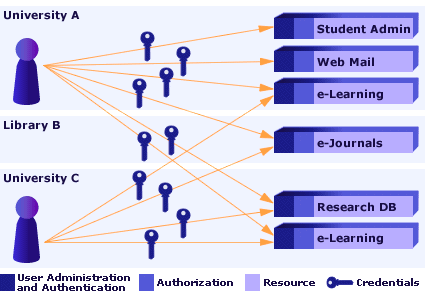
\includegraphics[width=\textwidth]{without-sso}
      \caption{Without SSO}
      \label{fig:without-sso}
    \end{subfigure}
    \hfill
    \begin{subfigure}{0.49\textwidth}
      \centering
      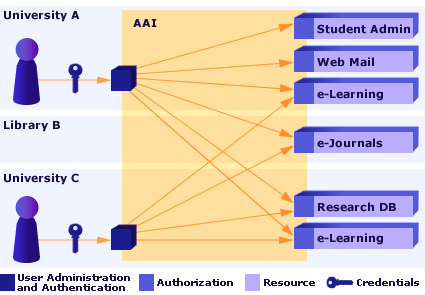
\includegraphics[width=\textwidth]{with-sso}
      \caption{With SSO}
      \label{fig:with-sso}
    \end{subfigure}
      \caption{Difference between accessing multiple resources with and without
      Single Sign-On (SSO). \\ \textit{Source:}
      \url{https://help.switch.ch/aai/about/introduction/}} 
      \label{fig:sso}
\end{figure}

Without SSO (see Fig.~\ref{fig:without-sso}), a user must register separately
with each resource they wish to access, typically receiving a new username and
password for each one. This results in users having to manage multiple sets of
credentials, one for each Resource, which can be cumbersome and inefficient.
Each Resource administrator must individually register and manage user accounts,
leading to duplicated efforts and potential security risks.

SSO simplifies the process of accessing multiple resources by using the concept
of federated identity management in the sign-up scenario depicted in
Fig.~\ref{fig:with-sso}:
 
\begin{enumerate}
\item A user registers only once with their Home Organization, such as a
university, or library, which is responsible for maintaining their credentials.

\item Authentication is always carried out by the Home Organization, which can
also provide additional information to the Resource upon request and user
consent. This means that with a single set of credentials, the user can access
all SSO-enabled Resources without needing to register separately for each one.
Resource operators benefit as well, as they no longer need to manage user
registrations; instead, they receive the necessary information directly from the
Home Organization. 

\item Finally, the requested resource makes access control decisions based on
the information retrieved from the Home Organization.
\end{enumerate}

\section{Authentication and Authorization Infrastructure}

An Authentication and Authorization Infrastructure (AAI) forms the technical and
organizational basis in order to perform SSO and federated identity management.
Participants in an AAI are called entities, whose relationships are depicted in
Fig.~\ref{fig:federation} and tasks are as follows:

\begin{figure}[htb]
    \centering
    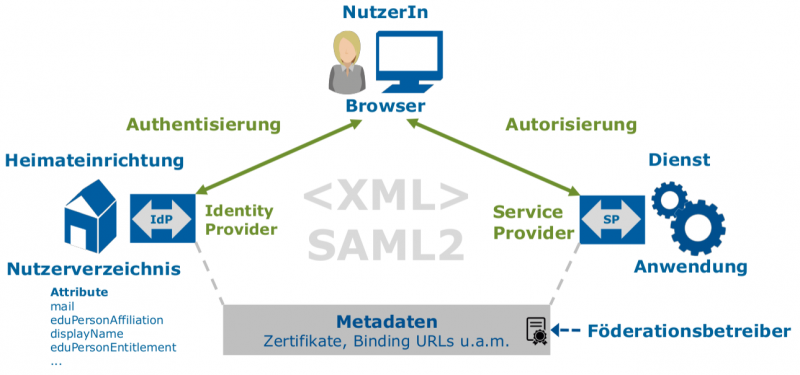
\includegraphics[width=0.8\textwidth]{federation_metadata}
    \caption{Schematic description of DFN-AAI: Entities and how they interact \\
    \textit{Source:} \url{https://doku.tid.dfn.de/de:aai:about}}
    \label{fig:federation}
  \end{figure}

\subsubsection*{Identity Provider (IdP)}
An Identity Provider handles user identity management and authentication
protocols. When a user attempts to access a protected resource, the IdP verifies
the user's identity based on the provided credentials (such as username and
password) or other authentication methods (like multifactor authentication). If
the authentication is successful, the IdP generates a security assertion
containing information about the user (attributes) and their permissions.

\subsubsection*{Service Provider (SP)}
A Service Provider hosts the applications or resources that users want to
access. It relies on the Identity Provider for user authentication and
authorization. When a user attempts to access a protected resource, the SP
redirects the user to the IdP for authentication. After successful
authentication, the IdP sends a security assertion to the SP. It then verifies
the assertion and grants the user access to the requested resource.

\subsubsection*{Attributes}
Attributes are user information which are included in the security assertion
issued by the Identity Provider. These attributes provide additional context
about the user's identity, roles, permissions, and other relevant information.
Attributes can include things like username, email address, role memberships,
group affiliations, entitlements, and custom attributes defined by the
organization. Service Providers use these attributes to make access control
decisions and personalize the user experience.

\subsubsection*{Security Assertion}
A security assertion is a digitally signed document issued by the Identity
Provider that contains information about the user's identity and permissions. It
typically includes attributes such as the user's unique identifier, username,
email address, roles, group memberships, and other relevant information. The
security assertion is sent to the Service Provider after the user successfully
authenticates, allowing the SP to make access control decisions based on the
user's attributes.

\subsection*{DFN AAI}
In the background of such infrastructures stands the exchange of metadata.
Hence, metadata has to be collected and provided in a central manner. This forms
one of the core functionalities of an AAI which is traditionally implemented
within the framework of national federations and is usually operated by the
respective research networks. In the case of the Federal Republic of Germany,
DFN-AAI~\cite{DFNAAI} managed by the DFN-Verein is used.

Types of metadata include both administrative (organization, contact data) and
technical data (service endpoints, certificates, etc.) that are required for the
entities to communicate with each other. An AAI must register the IdPs of
participating home organizations (educational and research institutions) as well
as participating service providers (content providers, e-learning platforms,
scientific services, etc.). The task of the respective federation is to maintain
these data records, keep them up to date and ensure that a secure and
trustworthy exchange of information takes place within the federation. A
federation acts as a Trusted Third Party, which ensures compliance with the
technical and legal framework conditions and thus establishes a relationship of
trust. 

\section{Shibboleth}
Shibboleth is an open-source software project developed and maintained by the
Shibboleth Consortium and provides a federated identity management framework
for web-based applications and services. It offers a set of software components
implementing an authentication and authorization system and is commonly used in
academic and organizational settings.

Shibboleth's infrastructure~\cite{cantor2005shibboleth} relies on the Security
Assertion Markup Language (SAML) standard for exchanging authentication and
authorization metadata between identity providers and service providers. SAML
provides a secure and interoperable framework for communication, ensuring
seamless identity federation across disparate systems and organizations. \\

\noindent The Shibboleth software stack consists of the following software
components:

\subsubsection*{Shibboleth Identity Provider (IdP)}
The IdP is a key component of the Shibboleth software stack and acts as a
trusted source for authenticating users and supplying data about them to service
providers. The IdP supports various authentication methods and protocols, such
as SAML and OpenID Connect, and allows organizations to define their own
authentication and authorization policies.

\subsubsection*{Shibboleth Service Provider (SP)}
The SP component integrates with web servers to enable web single sign-on and
controlled access to protected resources. It communicates with the IdP to
authenticate users and obtain their attributes, enforcing access control
policies based on the received information. The SP also supports various
federation standards, ensuring interoperability with IdPs from different
organizations.

\subsubsection*{Shibboleth Embedded Discovery Service (EDS)}
The EDS is a user interface component that provides a seamless and user-friendly
way for users to select their home organization for authentication. It is often
integrated with the login process, allowing users to easily locate and choose
their identity provider from a list of available options, simplifying the
authentication experience and improving usability. \\

\noindent For our use case, in which we want to enable SSO for a Service
Provider, we will focus on the installation and configuration of Shibboleth's SP
and EDS as described in Chapter~\ref{section:shibboleth}.



